%!TEX root = main.tex
\chapter{État de l'art}
\chaptertable

%\section{La visualisation et manipulation 3D collaborative sur web}

\section{Modélisation 3D collaborative sur le Web}

L'arrivée du web a bouleversé les usages liés à la collaboration sur des objets 3D. 
Les principes, les technologies, l'omniprésence du web en ont fait une plateforme 
de prédilection pour la visualisation et la manipulation d'objet 3D de haut niveau.   
Pour les projets d'\gls{AIC} ou de \gls{BIM}, la demande de traitement et la fidélité 
ont tendance à être plus élevés, particulièrement pour la représentation de dessins 
d'ingénierie ou de modèles d'architecture 3D. 
Les objets simples (primitives) ou les maillages optimisés pour le rendu temps-réel 
ne sont ni suffisants ni assez génériques pour être supporté par tous les 
processus liés à l'élaboration d'un produit. 
Plus les projets sont gros, plus ils dépendent d'une multitude de logiciels 3D --  
dont l'interopérabilité n'est pas garantie -- s'adressant chacun aux besoins d'une 
tâche spécifique. 
Chaque tâche (ex: modélisation \gls{CAO}, \textit{stress testing}\ldots) possède sa 
propre représentation des données qui peut varier selon les niveaux de 
sémantique attachés à la géométrie. 
Pour garder une trace de ces données et mettre en commun les données 
générées autour d'un produit, l'utilisation d'un \gls{PDM}/\gls{PLM} est 
souvent requise. Bien que certains outils de création d'objets 3D (par exemple 
Autodesk Revit) autorisent la synchronisation de fichier via leur dépôt à distance, 
ce n'est généralement pas applicable aux générations suivantes. 
En cela, une plateforme web pour un \gls{PDM}/\gls{PLM} à 
l'avantage d'être distribuée pour être accessible depuis un navigateur web ; avec 
un système d'édition hors-ligne, le téléversement peut s'avérer long et fastidieux.
De plus, les logiciels spécialisés pour la modélisation 3D, contrairement aux jeux 
multijoueurs, sont traditionnellement dédiés à un utilisateur unique sans 
représentation visuelle des autres opérateurs dans le même espace 3D. 
Ici encore, les principes d'accessibilité du web facilitent la création d'un espace 
virtuel 3D collaboratif pour la visualisation, la manipulation et l'échange de
données partagées. 
\subsection{HTML5 et au delà}
%TODO designing in context
%\cite{Dobos2015}

La collaboration en temps-réel est de plus en plus présente sur le web pour 
différents types de documents notamment 3D.
La revue sur la visualisation distribuée, effectuée par Grimstead et al. en 2005 
\cite{Grimstead2005}, indique que la plupart des systèmes sont conçus pour 
moins de cent 
utilisateurs simultanés et reposent sur un ou plusieurs serveurs pour supporter ces 
utilisateurs. 
Ils expliquent ce schéma par la volonté du fournisseur de service d'assurer une 
qualité de service et la sécurité du système. 
Les systèmes de \gls{RV} collaboratifs font exception à ce schéma où l'utilisation 
des réseaux \gls{P2P} est plus répandue pour supporter parfois plus d'un millier 
d'utilisateurs simultanés. 
Dans chacun des cas, chaque système a besoin d'un client adapté pour opérer de 
manière isolée sans inter-opérer avec les autre systèmes. 
C'est dans ce contexte qu'en 2011, Mouton et al. \cite{Mouton2011} présentent 
une analyse approfondie de l'état des environnements collaboratifs 3D, ciblant 
principalement la visualisation collaborative. 
Ils montrent l'apparition de la tendance à déporter les environnements collaboratifs 
sur le web grâce à l'évolution d'XMLHttpRequest en client-serveur et l'apparition du 
standard HTML5 comprenant un support avancé de l'audio et de la vidéo ainsi que 
plusieurs \gls{API} de stockage côté client (LocalStorage, IndexedDB). 
Les applications web revêtent plusieurs avantages par rapport aux applications 
natives sur mobiles ou aux logiciels autonomes. 
Cela repose principalement sur le fait que les navigateurs sont présents partout 
dans nos vies aujourd'hui (2017), incluant les téléphones intelligents et les 
tablettes qui les rendent indépendants des plateformes utilisées. 
Le déploiement sur le web ne requiert pas d'installation ou de mises à jour autre 
que celle du navigateur (en ne considérant que les applications sans greffon). 
La modification de l'application est gérée de manière centralisée par les serveurs 
qui distribuent l'application. 
Les éditeurs peuvent diffuser leur application à l'échelle mondiale instantanément  
et la mettre à disposition des utilisateurs sans dépendre d'un réseau de distribution 
autre qu'internet.

%Computer-Aided Engineering (CAE) Collaborative /


Parmi les solutions sans greffon (\textit{plugin less}), beaucoup sont développées 
pour faire de la modélisation 3D  et utilisent l'architecture client-serveur et le 
protocole 
\gls{WebSocket} pour effectuer la synchronisation entre les différents les clients 
collaborateurs. Quelques raisons peuvent expliquer cette situation :
\begin{enumerate}
	\item développement : connaissance du standard \gls{WebSocket} par les 
	développeurs (historique)
	\item gestion des données : simplification de la synchronisation des données 
	(centralisé)
	\item suivi de l'utilisateur : dépendance de l'utilisateur vis à vis de la connexion 
	au serveur et donc du service (engagement) 
\end{enumerate}

Parmi les solutions commerciales comme OnShape, Clara.io et TinkerCAD le 
choix de plateformes web dans l'infonuagique pour la modélisation \gls{CAO} est 
prépondérant souvent assorti d'un gestionnaire de version et d'une plateforme de 
diffusion des création.
OnShape est un service de modélisation 3D très riche dont l'objectif est de 
proposer une qualité équivalente des fonctionnalités de modeleurs autonomes 
(\textit{standalone}) professionnels, le tout de manière collaborative. Leur approche 
de la gestion de version développe le concept de micro version \cite{Baran2015}. 
Cette approche se retrouve dans les travaux de \cite{Lu2016} qui l'utilise gérer 
l'évolution de productions participatives liées à des tâches de modélisation 
3D en utilisant la créativité, l'intelligence et le savoir-faire 
d'un grand nombre de personnes en sous-traitance (\textit{crowdsourcing}). Le 
modeleur 3D Clara.io \cite{Houston2013} est plus généraliste. Il s'oriente 
davantage vers des fonctionnalités avancées de rendu 3D sur le \textit{cloud} en 
utilisant du lancer de rayons. 
Les fonctionnalités d'historisation et de collaboration proposées 
dans Clara.io restent très basiques (seulement annuler~/~refaire). TinkerCAD 
est aussi une plateforme de publication d'objets 3D pour faciliter l'accès à la 
conception d'objets 3D. TinkerCAD est une application destinée au grand 
public pour la conception et l'impression 3D. De ce fait, les fonctionnalités sont 
limitée à cause du métier, l'impression 3D et de la cible, grand public. La gestion 
de version est donc plus légère, similaire à celle proposée par Clara.io. 
OpenJSCAD, Verold Studio, Vectary sont d'autres 
exemples de modeleurs 3D moins connus avec des fonctionnalités proches de 
TinkerCAD.
Un peu à part, GrabCAD est une plateforme web plus orientée sur la gestion de 
données 3D \gls{CAO} (\gls{PLM}) qui possède un système de gestion de version 
performant et une système d'annotation et de visualisation collaborative.
Pour réduire l'empreinte mémoire des messages transmis lors de la collaboration 
sur le web, certains systèmes d'édition collaborative de contenu 3D utilisent une 
modélisation par surface implicite (BlobTree) \cite{Grasberger2013}. 
Les objets sont alors manipulés comme des géométries de construction de 
solides avec les opérations booléennes associées. 
Le Tableau \ref{table:encoding} résume les différents types 
d'encodage associé au type de modélisation 3D. 
\improve{tableau comparatif gestion historique ou versionning}
\improve{tableau comparatif de GrabCAD, OnShape, clara.io}
%
%\begin{table}[]
%	\centering
%	\caption{Comparaison de fonctionnalités entres modeleurs 3D basés web}
%	\label{my-label}
%	\begin{tabular}{@{}cccc@{}}
%		&  Client serveur & P2P &  Collaboratif\\ \midrule
%		Claro.io        & c        & g       & o       \\
%		GrabCAD                  & c        & g       & o       \\
%		OnShape &          &         &         \\
%		&          &         &         \\ \bottomrule
%	\end{tabular}
%\end{table}
\begin{table}[h]
	\centering
	\caption{Encodage des données transmises}
	\label{table:encoding}
	\begin{tabular}{@{}lcc@{}}\hline
		\textbf{Référence}& \textbf{Modélisation 3D}   & 
		\begin{tabular}[c]{@{}l@{}}\textbf{Encodage des}\\ 
			\textbf{modifications}\end{tabular} \\ \midrule
		\cite{Grasberger2013}        &      Blob (CSG)    & Fonction implicite        \\
		Clara.io \cite{Houston2013}               & Polygonale       &  Commande 
		interface     \\
		\cite{Mouton2014}                  & Polygonale       & Fonction paramétrique     \\
		OnShape \cite{Baran2015} &    Paramétrique      &     Microversion    \\
		cSculpt \cite{Calabrese2016} &      Polygonale    &    Fréquence spatiale  \\ 
		\bottomrule
	\end{tabular}
\end{table}

\subsection{Web 3D : deux approches}
La plateforme web possède certains avantages par rapport à des clients lourds. 
En effet, le développement de l'infonuagique a permis le développement de 
meilleures infrastructures de services. Du fait de ce développement, la création de 
plateformes collaboratives sur le web pour faire de la conception 3D est devenue 
non seulement faisable en termes de ressources mais également en termes de 
technologie. Il existe deux types d'approches pour créer du contenu web 2D ou 
3D. L'approche déclarative et l'approche impérative. La Figure \ref{fig:impdec} 
montre le pendant 3D pour chaque approche 2D. En 2D, les spécifications 
déclaratives (\gls{SVG}) et impératives (canvas) sont issues du \gls{HTML}5 alors 
qu'en 3D, les spécifications sont encore en évolution. 

\begin{figure}[hbt]
	\centering
	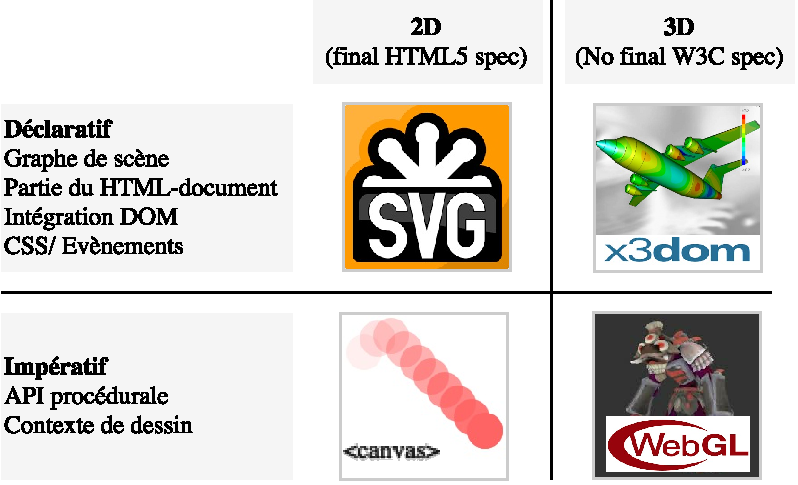
\includegraphics[width=0.7\columnwidth]{impdec}
	\caption{Déclaratif vs Impératif en 2D et en 3D sur le web}
	\label{fig:impdec}
\end{figure}

L'approche déclarative (Dec3D) s'intègre au \gls{DOM} et se 
focalise sur l'utilisation les technologies du web existantes comme CSS3, 
\gls{HTML}5 et l'Ajax. 
X3D est ainsi un format de fichier respectant le standard ISO \cite{X3D2011} pour 
représenter des scènes 3D interactives en XML, rétro-compatible avec VRML97. Il 
se différencie des formats de fichier type Collada en intégrant le comportement de 
la scène durant l'exécution en plus de la description du contenu 3D. Les deux 
bibliothèques les plus notables dérivées de ce standard sont X3DOM 
\cite{Behr2010} et XML3D \cite{Sons2010} : toutes les deux sont capables de 
supporter les récentes avancées de WebGL pour afficher une scène décrite dans 
le \gls{DOM} à l'intérieur d'un \textit{canvas} \gls{HTML}5. 
X3DOM essaye de respecter le standard X3D et ses concepts pour en permettre 
l'intégration du format dans le \gls{DOM}. De plus, X3DOM intègre le support 
d'élément \gls{HTML}, les évènements \gls{DOM} et de profils \acrshort{CSS} en 
supplément \cite{Sutter2015}. 
En comparaison avec X3DOM, XML3D a développé une extension à \gls{HTML}5 
pour décrire une scène 3D. 
L'utilisation d'un langage déclaratif basé sur XML comme X3D est bien 
adapté pour le contenu 3D utilise des données CAO/MAO ou WCS dans des 
applications \gls{SIG} car il peut être directement transformé (ex. XSLT) d'une 
représentation à une autre (tout comme le X3D peut être rendu dans un navigateur 
en utilisant X3DOM). 

L'approche déclarative est utilisée dans de nombreux travaux de visualisation 
scientifique 3D distribuée \cite{Jung2012} pour des données spatiales 
\cite{Stein2014} ou du rendu volumique \cite{Becher2012} par exemple. 
En manipulant directement les objets 3D à partir des éléments \gls{DOM}, grâce à 
sa structure bien connue, il est alors plus simple lors de la collaboration d'utiliser 
ces éléments \cite{Gadea2016} ou les évènements du \gls{DOM} \cite{Lowet2009} 
comme protocole de synchronisation de scènes. 
L'ajout de nombreux \textit{listeners} sur un document peut affecter les 
performances de parcours de l'arbre du \gls{DOM} notamment si une scène 
très peuplée.
%declarative XML- based languages such as X3D are suited well for SOAs in that 
%3D content, such as CAD/ CAM data or a given WCS response in a GIS 
%application, can be directly transformed, e.g. via an XSLT or similar transform, 
%from one representa- tion to another (such as an X3D world that can be rendered 
%in 
%real-time in the web browser using the X3DOM frame- work).

%TODO BIM CAD PLM 
%TODO Building Information Modeling: The Web3D Application for AEC 
%\cite{Campbell2007}
%TODO WEB3D, COLLABORATIVE DESIGN AND PLM Enrico Vezzetti (1), 
%Maria Grazia Violante (2)
%\info{webrtc collaborative visual analysis \cite{Li2015} }
%\info{webrtc medical \cite{Andrikos2015}}
%\info{webrtc x3dom \cite{Stein2014} \cite{Andrioti2015} }
%\info{webrtc webgl \cite{Desprat2015} \cite{Desprat2016} SAGE2 
%\cite{Marrinan2008} }

\begin{figure}[hbt]
	\centering
	\includegraphics[width=0.9\columnwidth]{webglstats.eps}
	\caption{Support de WebGL 1 (2014-2017) et WebGL 2 
		(2016-2017)}
	\label{fig:webglstats}
\end{figure}

Concernant l'approche impérative, la spécification WebGL 1.0 \cite{Khronos2011} 
proposée par le groupe Khronos permet aux navigateurs d'effectuer un rendu 3D 
grâce à une \gls{API} JavaScript adaptée de l'\gls{API} d'OpenGL~ES~2.0 
\cite{Khronos2007} en utilisant l'élément \textit{canvas} d'\gls{HTML}5. Cette 
spécification est supportée par la plupart des navigateurs traditionnels (Chrome 
depuis v49, Firefox depuis v52, Safari depuis v9.1, IE 11\footnote{Le contexte 
	WebGL est accessible depuis <<~\texttt{experimental-webgl}~>> au lieu de 
	<<~\texttt{webgl}~>>.\label{fn:webglcontext}}, Edge 14\textsuperscript{ 
	\ref{fn:webglcontext}} et Opera depuis v41) ainsi que les navigateurs mobiles 
	(iOS 
Safari depuis v9.3, Android Browser depuis v53 et Chrome for Android depuis v53) 
à l'exception d'Opera Mini\footnote{Données issues de 
	\url{http://caniuse.com/\#search=webgl}, consulté le 26/11/2016.}. La 
	spécification 
WebGL 2.0 \cite{Khronos2016} basée sur OpenGL~ES~3.0 \cite{Khronos2008}, 
déjà publiée en tant que brouillon, est en phase 
expérimentale\footnote{\url{http://caniuse.com/\#feat=webgl2} consulté le 
	26/11/2016}.\improve{add some example of coviz web} La Figure 
\ref{fig:webglstats} montre l'évolution du support de WebGL~1 et WebGL~2 durant 
ces dernières années sur les différentes plateformes possédant un navigateur 
web\footnote{Images capturées sur \url{https://webglstats.com/}. Les statistiques 
	sont collectées à partir de sites partenaires de \url{webglstats.com}. Ces sites 
	sont en 
	ciblent des néophytes de la WebGL possédant donc le matériel 
	dédié à la 3D en général. Consulté le 04/07/2017.}.

\section{Communication en temps-réel}
L'expression temps-réel est largement utilisé par des applications requérant une 
forme de temps de réponse rapide et réactif pour que l'utilisateur ait une bonne 
expérience.

L'exigence vis-à-vis des temps de réponse est de plus en plus 
grande pour deux raisons principales : les limitations humaines (mémoire et 
attention limitées 
à court terme) et les aspirations de l'être humain (besoin d'être en contrôle sur les 
machines). S'accroissant au gré de la technologie et aux attentes 
utilisateurs (rétro-compatibilité, temps de 
chargement), elle varie selon le domaine mais reste très assez prégnante sur le 
web en général. 
Par exemple, dans un domaine annexe comme le e-commerce, une étude réalisée 
en 2006 explique qu’une grande partie des internautes abandonnaient leurs achats 
en ligne si les pages mettaient 4 secondes ou plus à charger. De nos jours, ce 
délai a été réduit au quart de seconde pour les grandes entreprises du web. Jakob 
Nielsen \cite{Nielsen1993} indique trois temps de réponse limites concernant les 
temps de réponses :
\begin{itemize}
	\item \textit{0,1 seconde} donne une sensation de réponse instantanée, comme 
	si le 
	résultat avait été produit par l'utilisateur et non l'ordinateur. Ce niveau de temps 
	de réponse soutient la sensation de manipulation directe.\footnote{En IHM, la 
		manipulation directe correspond à un mode d'interaction au cours duquel les 
		utilisateurs font des actions sur les objets d'intérêt affichés dans l'interface 
		utilisateur en utilisant des actions physiques, incrémentales et réversibles 
		dont 
		les effets sont immédiatement visibles sur l'écran.} 
	\item \textit{1 seconde} garde le flux de pensées de l'utilisateur sans 
	interuption. 
	L'utilisateur peut ressentir un délai et par conséquent savoir que c'est la 
	machine qui génère le résultat ; l'utilisateur a quand même une impression de 
	contrôle sur l'expérience générale et peut de déplacer librement dans l'interface 
	sans attendre la machine. Ce degré de réactivité est impératif pour une bonne 
	navigation.
	\item \textit{10 secondes} conservent l'attention de l'utilisateur. Entre 1 et 10 
	secondes, l'utilisateur se sent dépendant de la machine, mais peut faire avec. 
	Au delà, l'utilisateur va commencer à penser à d'autres choses, rendant difficile 
	le retour à la tâche une fois que la machine répond.
\end{itemize} 

Dans le domaine de l'édition et la manipulation collaborative 
d'objets 3D, les contraintes abordées se situent à divers degrés : au chargement 
et lors des mises à jour. Le chargement concerne la phase de téléchargement de 
l'application web et des données relatives mais également d'affichage des 
modèles 3D sont spécifiques dans ce domaine car ils ont 
tendance à être lourds (structure de données 3D et métadonnées) à charger 
(contrairement au texte par exemple). Cette phase peut s'accorder des délais 
relativement long (1-10s) compte tenu du fait que l'utilisateur connaît en partie ces 
contraintes liées à la taille des objets 3D. Concernant les mises à jour, l'édition 
collaborative requiert un temps de réponse raisonnablement court est contraint par 
l'exactitude des calculs et le temps dans lequel le résultat est produit. Pour les 
mises à jour internes -- produites par l'utilisateur, actions sur l'interface -- on 
s'accordera sur un délai inférieur à 0,1 seconde dans cette thèse. 
Pour les mises à jour externes -- produites par les collaborateurs -- les latences 
réseaux rentrent en comptes (serveur, pairs\ldots) on s'accordera sur un délai 
entre 1 et 10 secondes dans cette thèse selon les degrés d'asynchronicité 
possibles. 

Un protocole de communication en temps-réel existe, il s'appelle \gls{RTP} et a 
été développé dans le but de faciliter la communication en temps-réel sur un 
réseau. Coexistant avec \gls{RTP}, le protocole \gls{RTCP} est utilisé pour 
transmettre des informations de contrôle à propos des données en temps-réelles. 
\gls{RTCP} transporte des données contenant des informations de contrôle et des 
informations statistiques concernant les flux de données et les connexions des 
destinataires qui permettent à l'expéditeur d'ajuster le flux en conséquence. Les 
protocoles \gls{RTP} et \gls{RTCP} sont principalement conçus pour la 
transmission de flux audio et vidéo, moins pour des données arbitraires comme 
des données 3D. Pour cette raison, leur utilisation est limitée dans le cadre des 
\gls{EVC} pour la modélisation 3D. 

Du fait de la variété des \glspl{EVC3D} existants, LE 
protocole de communication parfait pour tous les types d'environnement n'existe 
pas. 
Les besoins en communication qui se formulent souvent en termes de 
fiabilité de la livraison des messages et de l'ordonnancement des messages sont 
les variables d'ajustement en fonction des contraintes qu'imposent les limites de 
temps de réponse et de bande passante.

%
%
%	\subsection{Introduction}
%	\subsection{Les approches centralisées}
%	\subsection{Les approches décentralisées}
%	\subsection{Conclusion}

%\section{Systèmes d'édition collaborative}
%	\subsection{Le modèle de cohérence CCI}
%	\subsection{Les approches pour les données 3D}
%	\subsection{Conclusion}


\section{Les systèmes distribués orientés évènements pour la collaboration}

	\subsection{Introduction}
% old evenements et collaboration
La plupart des systèmes basés évènements sont très populaires lorsqu'il s'agit de 
collaboration. On retrouve par exemple la spécification d'évènements composites 
pour le support de la collaboration dans la conception logicielle \cite{Yuan2002} 
ou encore la définition de patrons de conception dédiés à la collaboration dans les 
architectures basées évènement \cite{Verginadis2009}. Dans ce dernier domaine 
Papageorgiou et al. \cite{Papageorgiou2011} proposent un assistant pour la 
création de ces patrons pour la collaboration en s'appuyant sur un système de 
recommandation basé sur le contexte qui utilisent une représentation sémantique 
(\gls{OWL}).

CoDesign est un exemple de \gls{framework} permettant de faire de la 
conception logicielle de manière collaborative \cite{Bang2010}. L'utilisation d'une 
architecture basée évènement permet à l'application d'être très extensible car très 
peu couplée. Chaque instance CoDesign intègre un intergiciel appelé CoWare en 
charge de la synchronisation de contenus édités de manière concurrentes sur les 
différentes instances CoDesign ainsi qu'un module chargé de notifier les 
architectes de situations de modélisation conflictuelles. Les conflits sont 
catégorisés de trois manières différentes. 
	
%	\subsection{Les évènements comme base du comportement réactif}
	\subsection{Systèmes Publish / Subscribe}

Le système \acrlong{PubSub} est un mécanisme basé sur le paradigme des 
messages qui est beaucoup utilisé en Event Processing. 
Les \textit{publishers} (ceux qui émettent des messages) et les \textit{subscribers} 
(ceux qui souscrivent) sont couplés de manière lâche. 
Autrement dit, le \textit{publisher} n'est pas forcément au courant de l'existence de 
ses \textit{subscribers} et n'a donc pas de contrainte forte le liant à ces derniers. 
De son côté, le \textit{subscriber} est souvent indifférent au \textit{publisher} qui lui 
fournit les évènements qui l'intéressent. 
%TODO expliquer la figure 

\begin{figure}[h]
	\centering
	\inputTikZ{1}{eps/tikz/pubsub}
	\caption{Architecture Publish-Subscribe}
	\label{fig:pubsub}
\end{figure}


Les modèles utilisant le paradigme 
\gls{PubSub} supportent naturellement une communication \textit{many-to-many} 
entre les \textit{publishers} et les \textit{subscribers}.  De cette manière, on permet 
un meilleur passage à l'échelle d'une application avec une topologie du réseau plus 
flexible. 
Hermes \cite{Pietzuch2002} est un intergiciel (\textit{middleware}) distribué basé 
évènements. 
Pour répondre à des besoins de mise à l'échelle, d'interopérabilité, de fiabilité, 
d'expressivité et d'utilisabilité, il s'appui sur un modèle \gls{PubSub} basé types et 
attributs. 
En spécifiant d'abord le type et ensuite en filtrant sur les attributs des 
évènements, ce modèle rend le routage des données intuitif pour le 
développement d'application distribuées à grande échelle comme le commerce en 
ligne (\textit{e-commerce}). 
Dans le cadre de la gestion de groupe, Scribe \cite{Castro2002} propose un 
système \gls{PubSub} pour gérer des groupes de souscripteurs et une architecture 
de communication \textit{multicast} nécessaire à grande échelle pour envoyer les 
évènements à tous les souscripteurs. 

En juin 2017, Leonardo Quernozy propose une rétrospective des systèmes 
\gls{PubSub} en \gls{P2P} massifs lors de la conférence DEBS'2017 à 
Barcelone. 
Les premières traces d'une telles architecture remontent à 1987 avec 
la publication de Birman et Joseph \cite{Birman1987} lorsqu'ils évoquent \og 
the ''News'' service in the ISIS system\fg{}:

\blockcquote{Birman1987}{
	\og\textit{ This service allows processes to enroll in a 
		system-wide news facility. Each subscriber receives a
		copy of any messages having a "subject" for which it 
		has enrolled in the order they were posted. Although 
		modeled after net-news, the news service is an active 
		entity that informs processes immediately on learning 
		of an event about which they have expressed interest.}\fg{}
}

Après cette publication les premiers systèmes \gls{PubSub} commencent à 
se développer. Le concept de routeur d'information est introduite par Oki et al. 
\cite{Oki1993} : un seul bus d'information pour tous les services, objets, données 
\ldots Les protocoles de communication ont une sémantique minimale, 
les objets (instances de classe) sont auto-descriptifs, i.e. ils sont 
capable d'introspection (service, opérations, attributs) pour adapter leur 
comportement au changement, les types peuvent être définis dynamiquement et 
la communication est anonyme. 
Puis l'apparition de solutions plus avancées sont apparues avec le projet 
GRYPHON d'IBM \cite{Banavar1999}, SIENA \cite{Carzaniga2000}, REBECA 
\cite{Parzyjegla2010} et également REDS , JEDI, PADRES présentés plus en 
détails dans \cite{Tarkoma2012}.
Ces différentes solutions ont été conçues comme des systèmes de gestion avec 
des gestionnaires d'évènements dédiées. Le passage à l'échelle est 
principalement effectué par un routage efficace des évènements (comme le 
filtrage d'évènements). Seuls quelques travaux ont utilisé le concept de 
\textit{clustering} par intérêt comme moyen afin de réduire le nombre de 
notifications d'évènement et éviter la surcharge. 
A partir des années 2000, les 
systèmes \gls{P2P} ont commencer à émerger avec 
l'apparition de Gnutella et consorts, les DHTs (Chord, Pastry, Kademlia) et  
Réseaux non-structurés (Cyclon, Scamp, ADH). Ces systèmes ayant pour 
objectifs de gérer des réseaux massifs, dynamiques (churn), résistants aux 
erreurs, et offrants des primitives de communications basiques.
Les réseaux P2P promettent alors des propriétés intéressantes pour les 
infrastructures logicielles comme les systèmes PubSub concernant le passage à 
l'échelle. Cependant, les systèmes PubSub d'alors reposent sur une connaissance 
totale du réseau pour être efficace, du fait de leur taille limitée. La connaissance 
globale de l'information ne peut être collectée dans un système à grande échelle, 
c'est pourquoi la décentralisation de l'information est nécessaire. La connaissance 
peut vite devenir viciée dans un système dynamique décentralisé ce qui implique 
de trouver une méthode efficace pour gérer la dynamicité.

	
	
	\subsubsection{Outils de monitoring et de benchmark}
	
\subsection{Domain Driven Design}
%\subsection{Domain Driven Design : lier le fonctionnel et le code}
	
	\gls{DDD} (ou Conception Pilotée par le Domaine) est une approche de 
	développement logicielle qui a pour objectif de définir une vision et un 
	\textbf{langage partagé} (\textit{ubiquitous language}) pour les personnes 
	impliquées dans la construction d'une application \cite{Evans2003}\info{Eric 
	Evans 
		Domain-driven Design: Tackling Complexity in the Heart of Software}. 
	
	Le but est de mettre l'accent principal d'un projet sur le domaine et la logique du 
	domaine en basant des conceptions complexes sur un modèle du domaine afin 
	d'initier une collaboration créative entre les experts techniques et les experts du 
	domaine pour raffiner itérativement un modèle conceptuel qui relève de 
	problèmes 
	spécifiques au domaine.
	Les différents concepts du \gls{DDD} sont listés en suivant :
	\begin{description}
		\item[Le contexte] est le cadre dans lequel un mot apparaît qui détermine sa 
		signification
		\item[Le domaine] est une ontologie, une influence, ou une activité. 
		L'étendue du sujet auquel l'utilisateur applique un programme est le domaine 
		du logiciel 
		\item[Le modèle] est un système d'abstractions qui décrit les aspects 
		sélectionnés du domaine et qui sont utilisés pour résoudre les problèmes liés 
		à ce domaine
		\item[Le langage partagé] est un langage structuré autour du modèle du 
		domaine utilisé par tous les membres de l'équipe pour faire référence aux 
		activités de l'équipe permettant d'éviter la redondance et les ambigüités dans 
		un contexte donné.
	\end{description}
	Le \gls{DDD} permet de connecter le modèle et son implémentation en offrant 
	plusieurs avantages:
	\begin{itemize}
		\item La plasticité du système est mise en avant par l'expression de règles 
		et de comportements qui facilitent les changements fréquents.
		\item L'accent mis sur l'identification des interactions dans le système 
		encourage la mise en \oe{}uvre d'une interface orientée tâches 
		(\textit{task-based UI}).
		\item La testabilité fonctionnelle est intégrée via les règles métier explicitées 
		et concentrées dans une couche spécifique de l'application. Cela les rend 
		plus facilement identifiable et testable automatiquement.
		\item La robustesse est améliorée face aux changements dans le SI.
	\end{itemize}
	
	Les notions plus détaillées qui se rapportent au \gls{DDD} sont présentées dans 
	\cite{Evans2003} et \cite{Vernon2013}.\info{source: 
		http://blog.octo.com/domain-driven-design-des-armes-pour-affronter-la-complexite/}
	
	Le \gls{DDD} a également l'avantage de fonctionner en harmonie avec les 
	principes de l'\gls{ES}. L'approche logicielle \gls{DDD} étant conçue pour refléter 
	les évènements se déroulant dans la réalité métier qui ne sont pas 
	interchangeables -- la plupart du temps. L'utilisation d'architectures 
	basées évènements est naturelle dans ce genre d'environnement. 
	
	Les disciplines liées à la 3D dans un contexte industrielles ont besoin de 
	pouvoir 
	communiquer sur un langage commun pour permettre à chacun des 
	intervenants 
	de s'exprimer dans la création du produit. Par exemple, la \gls{CAO} est très 
	utile 
	dans un contexte d'ingénierie par l'utilisation de quatre propriétés fondamentales 
	telles que l'historique, les fonctionnalités, la paramétrisation et le haut niveau de 
	contrainte.
	
	\paragraph{Programmation réactive}
	Les différents livres publiés par Vaughn s'attachent également à montrer la 
	nécessitée pour les différentes branche de l'informatique à proposer des 
	systèmes 
	pour robustes et flexibles face aux nouvelles demandent. La publication du 
	Manifeste Réactif encourage le développement de systèmes \og plus flexibles, 
	à 
	couplage faible et extensibles\fg{}.
	
\subsection{Command Query Responsability Segregation}
%	\subsection{Command Query Responsability Segregation : garantir de 
%	l'intégrité 
%	des données }
\label{sec:CQRS}
Introduit par Greg Young en 2009 \cite{Young2009}, \gls{CQRS} est un patron de 
conception qui repose sur le principe de séparation des composants de traitement 
métier de l'information (écriture) et de la restitution de l'information (lecture). Le 
cadre offert par ce principe permet de lever certaines contraintes d'architecture 
comme la (\textit{scalability}) en faisant apparaître de nouvelles forces : la gestion 
de la concurrence dans la collaboration sur des règles métier propre à la 
modélisation 3D dans des cadres d'application spécifiques. En effet, selon le type 
d'application des règles vont régir qui peut effectuer quelle type de modification ou 
quelles sont les modifications qui peuvent être acceptables dans un cas et non 
dans un autre.
Le caractère vicié (\textit{staleness}) d'une donnée dans un environnement 
collaboratif est récurrent. Une fois que la donnée a été montrée à un utilisateur, la 
même donnée peut être changée par un autre utilisateur, elle est altérée. 
\gls{CQRS} pallie cela en répondant aux besoins suivants :
\begin{itemize}
	\item En traitement/ écriture : besoins transactionnels, garantie de cohérence 
	(\textit{consistency}) des données, de normalisation.
	\item En consultation/lecture: dénormalisation, scalabilité. \info{ajouter au dico}
\end{itemize}

La plupart des architectures en couches ne font pas explicitement référence à ces 
problèmes. Le fait de tout sauvegarder dans une base de données centralisée peut 
être une étape dans la gestion de la collaboration mais l'altération des données est 
souvent exacerbée par l'utilisation de caches comme accélérateur de performance.

L'\textbf{immuabili\-té} en \gls{CQRS} est un concept clé qui prévient la  
modification de l'état interne d'une commande ou d'un évènement. Les 
commandes sont immuables car leur usage nécessite un envoi direct au domaine 
pour être traitées. Quant aux évènements, ils sont immuables car ils représentent 
ce qui s'est produit dans le passé (qu'on ne peut donc pas changer). \info{En ce 
qui concernent le \gls{CQRS} et l'\gls{ES}  finir la phrase à mettre dans l'ES}

\subsection{Event Sourcing}
%\subsection{Event Sourcing : certifier la fiabilité et traçabilité des données}
\label{sec:es}
L'\gls{ES} est une approche complémentaire au \gls{CQRS} pour gérer la 
concurrence des données et capturer l'intention de l'utilisateur. Ce patron de 
conception stocke les évènements en mode ajout seulement 
(\textit{append-only}) pour sauvegarder le résultat des commandes sur le 
domaine. Cela permet de conserver tous les changements qui ont mené à un 
état plutôt qu'uniquement l'état. Ce paradigme permet de recréer n'importe quel 
état d'un agrégat à partir de la liste d'évènements qu'on lui a appliqué. Cette 
liste représente une base la vérité du système\jp{pas clair}. 
\improve{improve}\gls{ES} permet de simplifier les tâches complexes dans des 
domaines complexes comme la 3D en ne requérant pas la synchronisation de 
modèle de données et du métier. 

L'\gls{ES} est souvent présent dans des architecture asynchrones qui ont 
l'avantage de pouvoir utiliser des queues de message, plusieurs bases de 
données et où la partie lecture est éventuellement consistante.
La plupart de la littérature concernant ce patron se trouve en ligne, dans des 
billets de blog, des présentations, ou de la documentation logicielle. La 
littérature académique est relativement réduite, souvent rapproché des travaux 
sur l'évolution de graphes. Cette section fournit un aperçu des différentes 
définitions données de l'\gls{ES} et du vocabulaire lié à ce patron de conception.

\textbf{Martin Fowler} Martin Fowler a été le premier à utiliser le terme 
d'\acrlong{ES} en 2005. Il définit l'\gls{ES} comme \og une série de 
changements 
de l'état d'une application\fg{}'.  \og série d'évènements capture tout ce qui est 
nécessaire à la reconstruction de l'état courant'\fg{}. Il voit les évènements 
comme 
immuables et le journal d'évènement (\textit{event log}) comme un stockage 
linéaire (\textit{append only store}) des évènements. Les évènements ne sont 
jamais supprimés, le seul moyen de l'''annuler'' consiste à effectuer générer un 
évènement rétroactif. Une fois qu'un évènement rétroactif est ajouté, 
l'évènement 
rétroactif agit à l'inverse de l'évènement précédent pour compenser ses effets. 
Dans ce billet, Fowler n'établit pas clairement la distinction entre les 
évènements 
et les commandes qui déclenchent ces évènements. Ce problème est 
considéré 
dans plusieurs travaux.

\textbf{Greg Young} Auteur renommé dans le domaine de l'\gls{ES}, Greg 
Young décrit l'\gls{ES} comme \og le stockage de l'état courant sous la forme 
d'une série d'évènements et la reconstruction de l'état du système en rejouant 
cette série d'évènements'\fg{}. D'après lui, le journal d'évènements a également 
un comportement linéaire : les évènements qui sont déjà arrivés ne peuvent 
être défaits. Ce que Fowler appelle évènements rétroactifs, Young le décrit 
comme des actions inverses.

\textbf{Udi Dahan} Udi Dahan est également un auteur de billets de blog 
prolifique sur les systèmes \gls{ES}. Dans sa définition de l'\gls{ES}, Dahan 
insiste sur le fait que ``l'état du modèle du domain est persisté comme un 
\textit{flux} d'évènements plutôt qu'un simple instantané''.


Les avantages et les inconvénients de l'approche \gls{ES}, incluant et discutant 
notamment ceux relevés par \cite{Klamer2013a}.
%
	\begin{figure}[!h]
		
		\centering
		\noindent
		\begin{tikzpicture}[node distance=2.5cm,
		every node/.style={ font=\scriptsize}, align=left,text width=5em,
		text centered,
		axis/.style={very thick, ->, >=stealth',yshift=-1cm}, draw]
		% Specification of nodes (position, etc.)
		
		\node (e1)		[event]          {Created Scene \\"MyScene" 1};
		\node (e2)	  	[event, right of=e1]          {Added Mesh "Bunny" 1 \\to Scene 
		1};
		\node (e3)	  	[event, right of=e2]          {Added Mesh \\"Teapot" 2  \\to 
		Scene 1};
		\node (e4)	  	[eventn, right of=e3]          {Translated \\Mesh 2 to 
		\{x:0,y:0,z:1\}};
		\draw[axis] (-1.3,0)  -- (12.5,0) node(xline)[]{~~~~~~~~~~~Temps};
		
		\end{tikzpicture}
		\caption{Transaction en Event-Sourcing}
		\label{fig:es-transaction}
	\end{figure}
	
	\begin{figure}[!h]
		\centering
		\noindent
		\begin{tikzpicture}[node distance=2.5cm,
		every node/.style={ font=\scriptsize}, align=center,text width=5em,
		text centered,
		axis/.style={very thick, ->, >=stealth',yshift=-1cm}, draw]
		% Specification of nodes (position, etc.)
		
		\node (e1)		[event]          {Created Scene \\"MyScene" 1};
		\node (e2)	  	[event, right of=e1]          {Added Mesh "Bunny" 1 \\to Scene 
		1};
		\node (e3)	  	[event, right of=e2]          {Added Mesh \\"Teapot" 2  \\to 
		Scene 1};
		\node (e4)	  	[event, right of=e3]          {Translated \\Mesh 2 to 
		\{x:0,y:0,z:1\}};
		\node (e5)	  	[eventc, right of=e4]          {Canceled translation on Mesh 2};
		\draw[axis] (-1.3,0)  -- (12.5,0) node(xline)[]{~~~~~~~~~~~Temps};
		\end{tikzpicture}
		\caption{Transaction avec compensation en Event-Sourcing}
		\label{fig:es-transaction-delete}
	\end{figure}
	
	
	\begin{figure}[t]
		\centering
		
		\subfloat[Sans la notion de snapshot]{
			\includegraphics[width=0.4\textwidth]{without-snapshot.eps}
			\label{fig:es-without-snapshot}
		}
		\subfloat[Avec la notion de snapshot]{
			\includegraphics[width=0.4\textwidth]{without-snapshot.eps}
			\label{fig:es-snapshot}
		}
		\caption{Snapshot en Event-Sourcing}
	\end{figure}
	
\subsubsection{Avantages}
L'\gls{ES} peut apporter beaucoup d'avantages à une application, notamment 
lorsque les besoins en traçabilité de l'information sont importants comme dans 
la modélisation collaborative de données 3D.
L'historique du système est accessible tout au long de la vie de l'application ce 
qui implique qu'il est non seulement possible d'accéder à l'état courant du 
système, mais également toutes les actions ayant mené jusqu'à cet état. C'est 
un avantage certain pour les système critiques, les applications d'Informatique 
Décisionnelle (\gls{BI}) ou les applications collaboratives. La pratique la plus 
courante est de proposer un système principal et d'ajouter une multitude de 
sous-systèmes qui enregistrent les différentes métriques (analyse d'un ou 
plusieurs axes, \textit{reporting} sur une propriété) du système principal. Avec 
l'\gls{ES}, il est toujours possible de regarder <<dans le passé>> et récupérer 
les données à partir de ce moment. Par comparaison, les avantages de 
l'\gls{ES} sur l'Active Record sont:
\begin{itemize}
	\item un journal complet de tous les changements d'état,
	\item une traçabilité et un débogage efficace,
	\item de très bonnes performances,
	\item pas de mapping objet-relationnel (ORM)\info{citer fowler's book}.
\end{itemize}

	
\paragraph{Exemple} 
Une revue de projet d'une scène est effectuée dans le cadre d'une application 
collaborative de modélisation 3D en ligne. Le chef de projet remarque qu'un 
objet a subi énormément de modifications par rapport aux autres. Il examine en 
particulier cet objet pour en connaître les causes. Voici deux exemples 
d'observations possibles : 1/ les spécifications ne sont pas assez claires 2/ 
deux collaborateurs sont opposés sur la façon de modifier l'objet. L'origine de 
ces changements identifiée, le chef de projet pourra alors intervenir et clarifier 
le sujet. \improve{style exemple}

\paragraph{Résolution} Avec un système classique, la fonctionnalité doit être 
créée pour enregistrer ce traitement puis être testée et implémentée (dans cet 
exemple, il en faudrait deux). Seulement après, un rapport pourra être délivré. 
Dans un environnement utilisant l'\gls{ES}, tous les évènements existent déjà 
donc les données sont déjà disponibles et ont seulement à être analysées 
(dans 
notre exemples, les informations sont inhérentes aux évènements). De plus, les 
évènements étant stockés depuis le début de la vie de l'application\jp{préciser : 
	début de la vie}, beaucoup plus de données peuvent être analysées. On 
	pourra par 
exemple demander toutes les modifications d'un objet depuis la dernière 
connexion d'un utilisateur pour lui communiquer visuellement les différences par 
rapport à sa dernière visite.



\subsubsection{Inconvénients}
Les performances de l'application peuvent être affectées par l'utilisation de 
l'\gls{ES}. En effet, pour récupérer l'état courant à partir de l'Event Store, il est 
nécessaire de le calculer à partir des évènements reçus.
A chaque évènement créé (et stocké), ce processus sera alourdi car ils ne 
peuvent être supprimés. Plus la pile d'évènements est longue, plus cela prend 
du temps (linéaire). On peut considérer d'une part que l'on a besoin des 
évènements que lorsque qu'une commande est effectuée\info{rehydratation d'un 
agrégat diff avec projection -> eventually consistence (proj = EC /rehy -> 
valides}.\unsure{Dans tous les autres cas l'utilisation de \textit{snapshots} 
permet de contrer proprement ce problème en offrant une forme dénormalisée 
de la donnée.} Un \gls{snapshot} est une capture de l'état de l'agrégat à un 
moment qui correspond à l'empilement d'évènements ayant mené à cet état. En 
créant un \gls{snapshot}, on évite de reconstruire un état à partir du début de la 
vie de l'agrégat; on empile les nouveaux évènements à partir de ce snapshot. 
L'utilisation du \gls{snapshot} est intéressante à partir du moment où la pile 
d'évènements devient plus lourde que le \gls{snapshot} lui-même. Il est donc 
important de bien déterminer la périodicité du déclenchement du \gls{snapshot} 
(temporelle ou selon le nombre d'évènements).

Le parcours des évènements se fait classiquement du premier au dernier 
(\textit{bottom-up}). Si on utilise les \gls{snapshot}, on peut se permettre de les 
parcourir dans l'autre sens (\textit{top-bottom}) jusqu'à trouver un \gls{snapshot} 
puis appliquer tous les évènements qui sont arrivés entre ce \gls{snapshot} et 
l'état courant. Dans le cas où l'on souhaite accéder à des données historiques 
plus anciennes que le dernier \gls{snapshot}, le second parcours fonctionne 
aussi. Cependant, elle doit être évitée pour ne pas créer de dépendance entre 
les \gls{snapshot}. Sans les snapshots le modèle peut encore varier 
<<~librement~>> tant que l'on sait comment lui appliquer un évènement passé. 
Le fait de travailler avec des \gls{snapshot} crée une dépendance des 
snapshots qui doivent intégrer les modifications du domaine. Une solution est 
de recalculer les snapshots quand le domaine est modifié mais cela reste 
coûteux (et à éviter).\info{versionning event -> retro compatibilité}


\subsubsection{Event sourcing vs command sourcing}
Les patrons de conception \gls{CS} et \gls{ES} sont strictement déterministes pour 
avoir une exactitude rigoureuse de ce qui se passe dans le système.

Un évènement représente quelque chose qui est arrivé dans le domaine. Un 
évènement appliqué sur un état, donne un nouvel état. 
La condition pour appliquer un pur déterminisme en \gls{ES} est la fonction 
suivante : \texttt{State $\rightarrow$ Event $\rightarrow$ State}. Cette fonction met 
en correspondance les (mêmes) entrées avec les (mêmes) sorties, on peut se 
reposer dessus pour reconstituer un état à n'important quel moment dans le 
temps. Le déterminisme est appliqué en assurant à l'évènement tous les 
informations lui permettant de faire la transition (i.e. sans effet de bord). 
L'évènement est alors considéré comme une encapsulation de toutes les 
informations pertinentes concernant la transition du système d'un état à l'autre.

Une commande va être déclenchée par l'utilisateur qui veut modifier le domaine. 
Une commande appliquée sur un état va produire un ou plusieurs évènements (qui 
ne sont pas forcément appliqués à l'état courant de l'application par la suite): 
\texttt{State $\rightarrow$ Command $\rightarrow$ Event list}

La différence principale entre un évènement et une commande réside donc dans 
l'\textbf{intention}. D'un point de vue fonctionnel, le \gls{CS} est un patron de 
conception lié à une décision qui produit plusieurs évènements, tandis que 
l'\gls{ES} se contente d'appliquer un changement à l'état courant. De plus, en 
\gls{ES}, l'évènement stocké a été produit par l'agrégat. 
La différenciation majeure des deux patrons de conception s'accentue lors 
l'interaction avec des systèmes externes. L'aspect fonctionnel de l'application de 
changement d'état de l'\gls{ES} al'avantage de permettre de reconstruire l'état sans 
effets de bord car elle ne travaille que sur l'état interne de l'application. 

Historiquement, l'\gls{ES} de Fowler dans ses premières versions ressemblait plus 
à du \gls{CS}. L'évolution de l'\gls{ES} a conduit à revoir ce patron théoriquement 
sous une forme fonctionnelle pure avec l'apparition de base de données comme 
EventStore ou le langage de programmation plus adaptés comme F\#.

Les deux patrons peuvent cohabiter si le \gls{CS} a un cadre d'action bien délimité 
et de les composants de l'architecture ont un couplage lâche afin que seuls les 
évènements produits par les agrégats ne modifient l'état interne de l'application. 


\subsection{Conclusion}

